\documentclass[11pt,class=report,crop=false]{standalone}
\usepackage[screen]{../python}


\begin{document}


%====================================================================
\chapitre{Gradient}
%====================================================================

\insertvideo{OUTxRsyLyeE}{partie 7.1. Dérivées partielles}

\insertvideo{7hDrbuz-nZQ}{partie 7.2. Gradient et géométrie}

\insertvideo{8GwXHvZcV3Q}{partie 7.3. Gradient et minimum/maximum}

\insertvideo{xQKw1xqNtvE}{partie 7.4. Différentiation automatique}

\insertvideo{7zf-oIerJsE}{partie 7.5. Gradient pour un réseau de neurones}



\objectifs{Le gradient est un vecteur qui remplace la notion de dérivée pour les fonctions de plusieurs variables. On sait que la dérivée permet de décider si une fonction est croissante ou décroissante. De même, le vecteur gradient indique la direction dans laquelle la fonction croît ou décroît le plus vite. Nous allons voir comment calculer de façon algorithmique le gradient grâce à la \og{}différentiation automatique\fg{}.}



%%%%%%%%%%%%%%%%%%%%%%%%%%%%%%%%%%%%%%%%%%%%%%%%%%%%%
\section{Dérivées partielles}

Pour une fonction de plusieurs variables, il existe une dérivée pour chacune des variables, qu'on appelle dérivée partielle. 

%----------------------------------------------------
\subsection{Définition}


\begin{definition}
Soit $f : \Rr^2 \to \Rr$. 
La \defi{dérivée partielle}\index{derivee partielle@dérivée partielle} $\frac{\partial f}{\partial x} (x_0,y_0)$ de $f$ par rapport à la variable $x$ au point $(x_0,y_0) \in \Rr^2$ est la dérivée en $x_0$ de 
la fonction d'une variable $x \mapsto f(x, y_0)$.

De même $\frac{\partial f}{\partial y} (x_0,y_0)$ est la dérivée partielle de $f$ par rapport à la variable $y$ au point $(x_0,y_0)$.


\end{definition}

Comme d'habitude et sauf mention contraire, nous supposerons que toutes les dérivées partielles existent.

Autrement dit, en revenant à la définition de la dérivée comme une limite :
 $$\frac{\partial f}{\partial x} (x_0,y_0) = \lim_{h \rightarrow 0} 
 \frac{f(x_0+h, y_0) - f(x_0,y_0)}{h}
\quad \text{ et } \quad 
\frac{\partial f}{\partial y} (x_0,y_0) = \lim_{h \rightarrow 0} 
 \frac{f(x_0, y_0+h) - f(x_0,y_0)}{h}.$$




Plus généralement, pour une fonction $f : \Rr^n \to \Rr$ de plusieurs variables,
$\frac{\partial f}{\partial x_i} (x_1,\ldots,x_n)$ est la dérivée partielle de $f$ par rapport à la variable $x_i$ au point $(x_1,\ldots,x_n) \in \Rr^n$.
C'est la dérivée en $x_i$ de la fonction d'une variable $x_i \mapsto f(x_1,\ldots,x_n)$ où l'on considère fixes les variables $x_j$ pour $j \neq i$.

\bigskip

\textbf{Notations.}
$$\frac{\partial f}{\partial x} (x,y) \quad \text{ et } \quad \frac{\partial f}{\partial y} (x,y)$$
sont les analogues de l'écriture $\frac{\dd f}{\dd x}(x)$ pour l'écriture de la dérivée lorsqu'il n'y a qu'une seule variable.
Le symbole \og{}$\partial$\fg{} se lit \og{}d rond\fg{}.
Une autre notation est $\partial_x f(x,y)$, $\partial_y f(x,y)$ ou bien encore $f'_x (x,y)$, $f'_y (x,y)$.




\bigskip

\begin{remarque*}
Pour une fonction d'une variable $f : \Rr \to \Rr$,
on distingue le nombre dérivé $f'(x_0)$ et la fonction dérivée $f'$ définie par $x \mapsto f'(x)$. Il en est de même avec les dérivées partielles. Pour $f : \Rr^2 \to \Rr$ :
\begin{itemize}
  \item $\displaystyle \frac{\partial f}{\partial x} (x_0,y_0)$ et $\displaystyle \frac{\partial f}{\partial y} (x_0,y_0)$
  sont des nombres réels.
  
  \item $\displaystyle \frac{\partial f}{\partial x}$ et $\displaystyle \frac{\partial f}{\partial y}$ sont des fonctions de deux variables, par exemple :
$$\begin{array}{cccc}
 \dfrac{\partial f}{\partial x} : & \Rr^2 & \longrightarrow & \Rr \\
                                 & (x,y) & \longmapsto & \dfrac{\partial f}{\partial x} (x,y)
\end{array}$$
\end{itemize}
\end{remarque*}



%----------------------------------------------------
\subsection{Calculs}

La calcul d'une dérivée partielle n'est pas plus compliqué que le calcul d'une dérivée.

\textbf{Méthode.}
Pour calculer une dérivée partielle par rapport à une variable, il suffit de dériver par rapport à cette variable en considérant les autres variables comme des constantes.


\begin{exemple}
Calculer les dérivées partielles de la fonction 
$f : \Rr^2 \to \Rr$ définie par $f(x,y)=x^2e^{3y}$.

\medskip
\emph{Solution.}

Pour calculer la dérivée partielle $\frac{\partial f}{\partial x}$, par rapport à $x$, on considère que $y$ est une constante et on dérive $x^2e ^{3y}$ comme si c'était une fonction de la variable $x$ uniquement :
$$\frac{\partial f}{\partial x}(x,y) =2xe ^{3y}.$$
Pour l'autre dérivée  $\frac{\partial f}{\partial y}$, on considère que $x$ est une constante et on dérive $x^2e ^{3y}$ comme si c'était une fonction de $y$ :
$$\frac{\partial f}{\partial y}(x,y) = 3x^2e ^{3y}.$$
\end{exemple}



\begin{exemple}
Pour $f : \Rr^3 \to \Rr$ définie par $f(x,y,z)=\cos (x+y^2)e^{-z}$ on a :
\begin{align*}
\frac{\partial f}{\partial x}(x,y,z) = -\sin(x+y^2)e^{-z}, \\
\frac{\partial f}{\partial y}(x,y,z) = -2y\sin(x+y^2)e^{-z}, \\
\frac{\partial f}{\partial z}(x,y,z) = -\cos(x+y^2)e^{-z}.
\end{align*}
\end{exemple}


\begin{exemple}
Soit $f :\Rr^n \to \Rr$ définie par 
$f(x_1,\ldots,x_n) = x_1^2+x_2^2+\cdots + x_n^2$,
alors pour $i=1,\ldots,n$ :
$$\frac{\partial f}{\partial x_i}(x_1,\ldots,x_n) = 2x_i.$$
\end{exemple}


%----------------------------------------------------
\subsection{Interprétation géométrique}


Pour une fonction d'une variable, la dérivée est la pente de la tangente au graphe de la fonction (le graphe étant alors une courbe). Pour une fonction de deux variables $(x,y) \mapsto f(x,y)$, les dérivées partielles indiquent les pentes au graphe de $f$ selon certaines directions (le graphe étant ici une surface). Plus précisément :

\begin{itemize}
  \item $\frac{\partial f}{\partial x} (x_0,y_0)$ est la pente du graphe de $f$
 en $(x_0,y_0)$ suivant la direction de l'axe $(Ox)$.
 En effet cette pente est celle de la tangente à la courbe $z = f(x,y_0)$ et est donnée par la dérivée de $x \mapsto f(x,y_0)$ en $x_0$, c'est donc bien $\frac{\partial f}{\partial x} (x_0,y_0)$.
 
 \item $\frac{\partial f}{\partial y} (x_0,y_0)$ est la pente du graphe de $f$
 en $(x_0,y_0)$ suivant la direction de l'axe $(Oy)$.
 

\end{itemize}

 
 
\bigskip 
Sur la figure de gauche, la dérivée partielle  $\frac{\partial f}{\partial x}$ indique la pente de la tranche parallèle à l'axe $(Ox)$\couleurnb{ (en orange)}{}. Sur la figure de droite, la dérivée partielle  $\frac{\partial f}{\partial y}$ indique la pente de la tranche parallèle à l'axe $(Oy)$\couleurnb{ (en vert)}{}.


\myfigure{0.75}{
  \tikzinput{fig-calculdiff-04}
  \tikzinput{fig-calculdiff-05}
} 





%%%%%%%%%%%%%%%%%%%%%%%%%%%%%%%%%%%%%%%%%%%%%%%%%%%%%
\section{Gradient}

Le gradient est un vecteur dont les coordonnées sont les dérivées partielles. Il a de nombreuses applications géométriques car il donne l'équation des tangences aux courbes et surfaces de niveau. Surtout, il indique la direction dans laquelle la fonction varie le plus vite.

%----------------------------------------------------
\subsection{Définition}

\begin{definition}
Soit $f : \Rr^2 \to \Rr$ une fonction admettant des dérivées partielles.
Le \defi{gradient}\index{gradient} de $f$ en $(x_0,y_0) \in \Rr^2$, noté 
$\grad f (x_0,y_0)$, est le vecteur :
$$\grad f (x_0,y_0) =
\begin{pmatrix} \dfrac{\partial f}{\partial x} (x_0,y_0)\\[2ex] \dfrac{\partial f}{\partial y}(x_0,y_0)\end{pmatrix}.$$
\end{definition}

Les physiciens et les anglo-saxons notent souvent $\nabla f (x,y)$ pour $\grad f (x,y)$. Le symbole $\nabla$ se lit \og{}nabla\fg{}.


Plus généralement, pour $f : \Rr^n \to \Rr$, le gradient de $f$ en $(x_1,\ldots,x_n) \in \Rr^n$ est le vecteur :
$$\grad f (x_1,\ldots,x_n) =
\begin{pmatrix} \dfrac{\partial f}{\partial x_{1}} (x_1,\ldots,x_n)\\ \vdots \\ \dfrac{\partial f}{\partial x_n}(x_1,\ldots,x_n)\end{pmatrix}.$$



\begin{exemple}
\sauteligne
\begin{itemize}
\item $f(x,y) = x^2y^3$, $\grad f (x,y) =  \begin{pmatrix}2xy^3\\3x^2y^2\end{pmatrix}$. Au point $(x_0,y_0)=(2,1)$, $\grad f (2,1) =  \begin{pmatrix}4\\12\end{pmatrix}$.

\item $f(x,y,z) = x^2\sin(yz)$, $\grad f (x,y,z) = \begin{pmatrix} 2x\sin(yz) \\ x^2z \cos(yz) \\ x^2y\cos(yz) \end{pmatrix}$.

\item $f(x_1,\ldots,x_n)= x_1^2+x_2^2+\cdots + x_n^2$, $\grad f (x_1,\ldots,x_n) =  \begin{pmatrix}2x_1\\ \vdots \\2x_n\end{pmatrix}$.
\end{itemize}
\end{exemple}

\begin{remarque*}
Le gradient est un élément de $\Rr^n$ écrit comme un vecteur colonne. Parfois, pour alléger l'écriture, on peut aussi l'écrire sous la forme d'un vecteur ligne.
\end{remarque*}

%----------------------------------------------------
\subsection{Tangentes aux lignes de niveau}


Soit $f : \Rr^2 \to \Rr$ une fonction différentiable. On considère les lignes de niveau $f(x,y)=k$.


\begin{proposition}
\index{lignes de niveau}
Le vecteur gradient $\grad f(x_0,y_0)$ est orthogonal à la ligne de niveau de $f$ passant au point $(x_0,y_0)$. 
\end{proposition}


Sur ce premier dessin, sont dessinés la ligne de niveau passant par le point $(x_0,y_0)$ \couleurnb{(en rouge)}{}, un vecteur tangent $v$ en ce point et la tangente à la ligne de niveau\couleurnb{ (en vert)}{}. 
Le vecteur gradient est un vecteur du plan qui est orthogonal à la ligne de niveau en ce point\couleurnb{ (en bleu)}{}.


\bigskip

\myfigure{0.8}{
  \tikzinput{fig-gradient-02}
}

À chaque point du plan, on peut associer un vecteur gradient. Ce vecteur gradient est orthogonal à la ligne de niveau passant par ce point. Nous verrons juste après comment savoir s'il est orienté \og{}vers le haut\fg{} ou \og{}vers le bas\fg{}. 

\myfigure{0.8}{
  \tikzinput{fig-gradient-01}
}

Dans le cadre de notre étude, nous nous intéressons à l'équation de la tangente.
\begin{proposition}
\index{tangente}
Au point $(x_0,y_0)$, l'équation de la tangente à la ligne de niveau de $f$ est :
$$\frac{\partial f}{\partial x}(x_0,y_0)(x-x_0)+\frac{\partial f}{\partial y}(x_0,y_0)(y-y_0)=0$$
pourvu que le gradient de $f$ en ce point ne soit pas le vecteur nul.
\end{proposition}



\begin{exemple}[Tangentes à une ellipse]
Trouver les tangentes à l'ellipse $\mathcal{E}$ d'équation $\frac{x^2}{a^2}+\frac{y^2}{b^2} = 1$.

\myfigure{0.7}{
  \tikzinput{fig-gradient-03}
}

Cette ellipse $\mathcal{E}$ est la ligne de niveau $f(x,y)=1$ de la fonction
$f(x,y) = \frac{x^2}{a^2}+\frac{y^2}{b^2}$. 
Les dérivées partielles en $(x_0, y_0)$ sont :
$$\frac{\partial f}{\partial x}(x_0,y_0) = \frac{2x_0}{a^2} \qquad \text{ et } \qquad \frac{\partial f}{\partial y}(x_0,y_0) = \frac{2y_0}{b^2}.$$
L'équation de la tangente à l'ellipse $\mathcal{E}$ en ce point est donc :
$$\frac{2x_0}{a^2}(x-x_0)+\frac{2y_0}{b^2}(y-y_0)=0.$$
Mais comme $\frac{x_0^2}{a^2}+\frac{y_0^2}{b^2} = 1$, l'équation de la tangente se simplifie en $\displaystyle \frac{x_0}{a^2}x + \frac{y_0}{b^2} y = 1$.
\end{exemple}


%----------------------------------------------------
\subsection{Lignes de plus forte pente}
 
Considérons les lignes de niveau $f(x,y)=k$ d'une fonction $f : \Rr^2 \to \Rr$.
On se place en un point $(x_0,y_0)$. On cherche dans quelle direction se déplacer pour augmenter au plus vite la valeur de $f$.
 
\begin{proposition}
Le vecteur gradient $\grad f(x_0,y_0)$ indique la direction de plus grande pente à partir du point $(x_0,y_0)$.
\end{proposition}


Autrement dit, si l'on veut, à partir d'un point donné $(x_0,y_0)$ de niveau $a$, passer au niveau $b>a$ le plus vite possible alors il faut démarrer en suivant la direction du gradient $\grad f(x_0,y_0)$. 

\myfigure{1}{
  \tikzinput{fig-gradient-05}
}

Comme illustration, un skieur de descente, voulant optimiser sa course, choisira en permanence de s'orienter suivant la plus forte pente, c'est-à-dire dans le sens opposé au gradient. 
 
%----------------------------------------------------
\subsection{Dérivée directionnelle}
 
Pour prouver que le gradient indique la ligne de la plus grande pente, nous avons besoin de généraliser la notion de dérivée partielle. Ce passage est plus technique et peut être ignoré en première lecture.

Soit $v=\left(\begin{smallmatrix}h\\k\end{smallmatrix}\right)$ un vecteur du plan.
La \defi{dérivée directionnelle} de $f$ suivant le vecteur $v$ en $(x_0,y_0)$ est le nombre :
$$D_v f(x_0,y_0) = h\frac{\partial f}{\partial x}(x_0,y_0)
 +k\frac{\partial f}{\partial y}(x_0,y_0).$$
 
 
La dérivée directionnelle correspond à la pente de la fonction pour la tranche dirigée par le vecteur $v$.

 \myfigure{0.8}{
   \tikzinput{fig-calculdiff-06}
 } 
 
Remarque : pour $v=\left(\begin{smallmatrix}1\\0\end{smallmatrix}\right)$
alors $D_v f(x_0,y_0) = \frac{\partial f}{\partial x}(x_0,y_0)$ et pour 
$v=\left(\begin{smallmatrix}0\\1\end{smallmatrix}\right)$
alors $D_v f(x_0,y_0) = \frac{\partial f}{\partial y}(x_0,y_0)$.


On rappelle que le \defi{produit scalaire} de deux vecteurs $u=\left(\begin{smallmatrix}x\\y\end{smallmatrix}\right)$ et 
$v=\left(\begin{smallmatrix}x'\\y'\end{smallmatrix}\right)$
est donné par 
$$\langle u \mid v \rangle = xx' + yy'.$$
On sait que le produit scalaire se calcule aussi géométriquement par :
$$\langle u \mid v \rangle = \|u\|\cdot \|v\| \cdot \cos(\theta)$$
où $\theta$ est l'angle entre $u$ et $v$.

 \myfigure{1}{
   \tikzinput{fig-scalaire}
 } 


Ainsi, on peut réécrire la dérivée directionnelle sous la forme :
$$D_v f(x_0,y_0) = \langle \grad f (x_0,y_0) \mid v \rangle.$$

 
On peut maintenant prouver que le gradient indique la ligne de plus grande pente.
 
\begin{proof}
La dérivée suivant le vecteur non nul $v$ au point $(x_0,y_0)$ décrit la variation de $f$ autour de ce point lorsqu'on se déplace dans la direction $v$. 
La direction selon laquelle la croissance est la plus grande est celle du gradient de $f$. En effet,
$$D_{v}f(x_0,y_0)=\langle \grad f(x_0,y_0) \mid v\rangle=
\| \grad f(x_0,y_0) \| \cdot \| v \| \cdot \cos \theta$$
où $\theta$ est l'angle entre le vecteur $\grad f(x_0,y_0)$ et le vecteur $v$.
Le maximum est atteint lorsque l'angle $\theta=0$, c'est-à-dire lorsque $v$ pointe dans la même direction que $\grad f(x_0,y_0)$.
\end{proof}


%----------------------------------------------------
\subsection{Surface de niveau}

Les résultats présentés ci-dessus pour les fonctions de deux variables se généralisent aux fonctions de trois variables ou plus.
Commençons avec trois variables et une fonction $f:\Rr^3 \to \Rr$.
Rappelons qu'un plan de $\Rr^3$ passant par $(x_0,y_0,z_0)$ et de vecteur normal 
$n=(a,b,c)$ a pour équation cartésienne :
$$a(x-x_0)+b(y-y_0)+c(z-z_0) = 0.$$


De même qu'il existe une droite tangente pour les lignes de niveau, il existe un \defi{plan tangent} à une surface de niveau.


\begin{proposition}
Le vecteur gradient $\grad f(x_0,y_0,z_0)$ est orthogonal à la surface de niveau de $f$ passant au point $(x_0,y_0,z_0)$. Autrement dit,
l'équation du plan tangent à la surface de niveau de $f$ en $(x_0,y_0,z_0)$ est 
$$\frac{\partial f}{\partial x}(x_0,y_0,z_0)(x-x_0)
+\frac{\partial f}{\partial y}(x_0,y_0,z_0)(y-y_0)
+\frac{\partial f}{\partial z}(x_0,y_0,z_0)(z-z_0)
 = 0 $$
pourvu que le gradient de $f$ en ce point ne soit pas le vecteur nul.
\end{proposition}


\myfigure{1}{
  \tikzinput{fig-gradient-07}
}


Plus généralement pour $f : \Rr^n \to \Rr$, $\grad f (x_1,\ldots,x_n)$ est orthogonal à l'espace tangent à
l'hypersurface de niveau $f=k$ passant par le point $(x_1,\ldots,x_n)\in\Rr^n$ et 
ce vecteur gradient $\grad f(x_1,\ldots,x_n)$ indique la direction de plus grande pente à partir du point $(x_1,\ldots,x_n)$.



%----------------------------------------------------
\subsection{Calcul approché}

Rappelez-vous que la dérivée nous a permis de faire des calculs approchés, par exemple pour estimer $\sqrt{1.01}$ sans calculatrice (voir le chapitre \og{}Dérivée\fg{}).
Voici, en deux variables, l'analogue de la formule pour une variable : 
$$f(x_0+h,y_0+k) \simeq f(x_0,y_0) + h\frac{\partial f}{\partial x}(x_0,y_0)
+k\frac{\partial f}{\partial y}(x_0,y_0).$$
Cette approximation est valable pour $h$ et $k$ petits.

L'interprétation géométrique est la suivante : 
on approche le graphe de $f$ en $(x_0,y_0)$ par le plan tangent au graphe en ce point. Sur la figure ci-dessous sont représentés : le graphe de $f$\couleurnb{ (en rouge)}{}, le plan tangent au-dessus du point $(x_0,y_0)$\couleurnb{ (en bleu)}{}. La valeur $z_1 = f(x_0+h,y_0+k)$ est la valeur exacte donnée par le point de la surface au dessus de $(x_0+h,y_0+k)$. On approche cette valeur par $z_2 = f(x_0,y_0) + h\frac{\partial f}{\partial x}(x_0,y_0)
+k\frac{\partial f}{\partial y}(x_0,y_0)$ donnée par le point du plan tangent au dessus de $(x_0+h,y_0+k)$. 


\myfigure{1}{
  \tikzinput{fig-gradient-10}
}


\begin{exemple}
Valeur approchée de $f(1.002, 0.997)$ si $f(x,y) = x^2y$.
\bigskip

\emph{Solution.}
Ici $(x_0,y_0) = (1,1)$, $h = 2 \times 10^{-3}$, $k = -3 \times 10^{-3}$,
$\frac{\partial f}{\partial x}(x,y) = 2xy$, $\frac{\partial f}{\partial y}(x,y) = x^2$, donc $\frac{\partial f}{\partial x}(x_0,y_0) = 2$, $\frac{\partial f}{\partial y}(x_0,y_0) = 1$. Ainsi
$$f(1+h,1+k) \simeq f(1,1) + 2h + k$$
donc 
$$f(1.002, 0.997) \simeq 1 + 2 \times 2 \times 10^{-3} - 3 \times 10^{-3} \simeq 1.001.$$
Avec une calculatrice, on trouve $f(1.002, 0.997) = 1.000992$ : l'approximation est bonne.
\end{exemple}


%----------------------------------------------------
\subsection{Minimum et maximum}

\begin{definition}
\index{minimum!local}
Soit $f : \Rr^2 \to \Rr$.
\begin{itemize}
  \item La fonction $f$ admet un \defi{minimum local} en $(x_0,y_0)$ s'il existe un disque $D$ centré en ce point tel que 
$$ f(x,y) \ge f(x_0,y_0) \quad \text{ pour tout } (x,y) \in D.$$
  \item La fonction $f$ admet un \defi{maximum local} en $(x_0,y_0)$  pour lequel 
$$f(x,y) \le f(x_0,y_0) \quad \text{ pour tout } (x,y) \in D.$$
  \item On parle d'un \defi{extremum local} pour un minimum ou un maximum local.
\end{itemize}
\end{definition}

% [[dessins 3D min/max]]

\begin{exemple}
L'exemple type de minimum est celui de la fonction $f(x,y)=x^2+y^2$ en $(0,0)$.
Voici son graphe et ses lignes de niveau.

\begin{center}
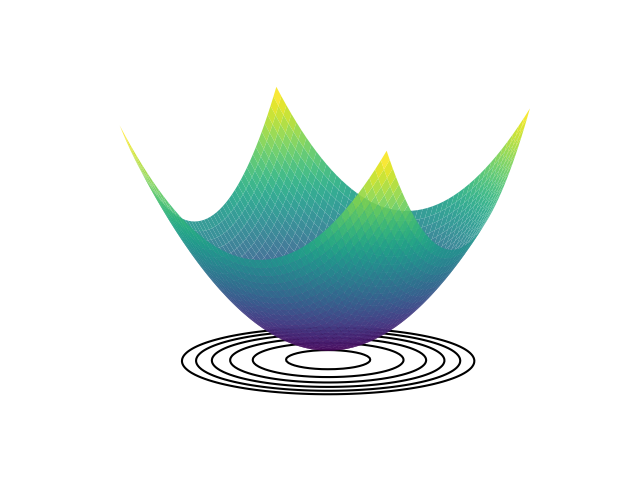
\includegraphics[scale=\myscale,scale=0.7]{figures/gradient-surface-1a}
\end{center}


La fonction $f(x,y) = -x^2-y^2$ admet, elle, un maximum en $(0,0)$.
\begin{center}
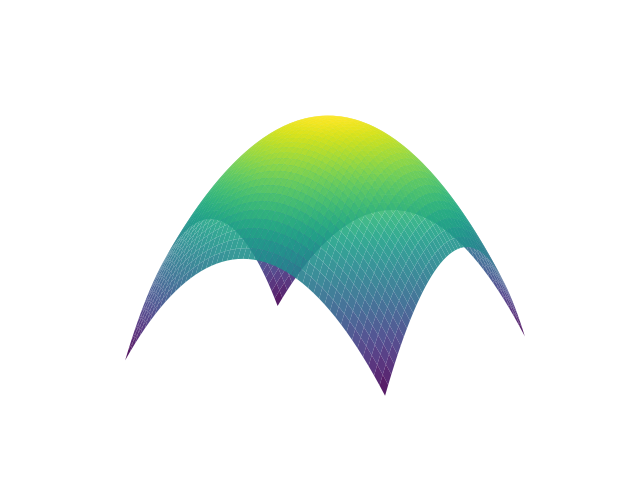
\includegraphics[scale=\myscale,scale=0.7]{figures/gradient-surface-2}
\end{center}

\end{exemple}

\begin{proposition}
Soit $f : \Rr^2 \to \Rr$. Si $f$ admet un minimum ou un maximum local en $(x_0,y_0)$ alors le gradient est le vecteur nul en ce point, autrement dit :
$$
\frac{\partial f}{\partial x}(x_0,y_0) = 0 
\quad \text{ et  }\quad
\frac{\partial f}{\partial y}(x_0,y_0) = 0.
$$
\end{proposition}

\begin{proof}
Prenons le cas d'un minimum local.
La fonction d'une variable $x \mapsto f(x, y_0)$ admet aussi un minimum en $x_0$ donc sa dérivée est nulle en $x_0$, c'est-à-dire $\frac{\partial f}{\partial x}(x_0,y_0) = 0$. De même $y \mapsto f(x_0, y)$ admet un minimum en $y_0$ donc $\frac{\partial f}{\partial y}(x_0,y_0) = 0$. 
\end{proof}


Dans la suite du cours nous chercherons les points pour lesquels une fonction donnée présente un minimum local.
D'après la proposition précédente, ces points sont à chercher parmi les points en lesquels le gradient s'annule. On dira que $(x_0,y_0)$ est un \defi{point critique}\index{point critique} de $f$ si
les deux dérivées partielles $\frac{\partial f}{\partial x}(x_0,y_0)$ et $\frac{\partial f}{\partial y}(x_0,y_0)$ s'annulent simultanément.

\begin{exemple}
Chercher les points en lesquels $f(x,y) = x^2-y^3+xy$ peut atteindre son minimum.

\textbf{Recherche des points critiques.}
On calcule 
$$\frac{\partial f}{\partial x}(x,y) = 2x+y 
\quad \text{ et } \quad 
\frac{\partial f}{\partial y}(x,y) = -3y^2+x.$$
On cherche les points $(x,y)$ en lesquels les deux dérivées partielles s'annulent.
Par l'annulation de la première dérivée, on a $2x+y=0$ donc $y=-2x$.
Par l'annulation de la seconde dérivée, on a $-3y^2+x=0$ ce qui donne par substitution
$-12x^2+x=0$, ainsi $x(-12x+1)=0$.
Donc soit $x=0$ et alors on a $y=0$, soit $x=\frac1{12}$ et alors $y=-\frac16$.
Bilan : il y a deux points critiques :
$$\left(0,0\right) \quad \text{ et } \quad \left(\frac1{12},-\frac16\right).$$

\textbf{\'Etude du point critique $(0,0)$.}
On a $f(0,0)=0$ mais on remarque que $f(0,y)=-y^3$ qui peut être négatif ou positif (selon le signe de $y$ proche de $0$), donc en $(0,0)$ il n'y a ni minimum ni maximum.

\textbf{\'Etude du point critique $(\frac1{12},-\frac16)$.}
Il existe un critère (que l'on ne décrira pas ici) qui permet de dire qu'en ce point $f$ admet un minimum local.

Sur le dessin ci-dessous, le minimum est situé à l'intérieur du petit ovale, l'autre point critique en $(0,0)$ correspond à l'intersection de la ligne de niveau $f=0$ avec elle-même.
\begin{center}
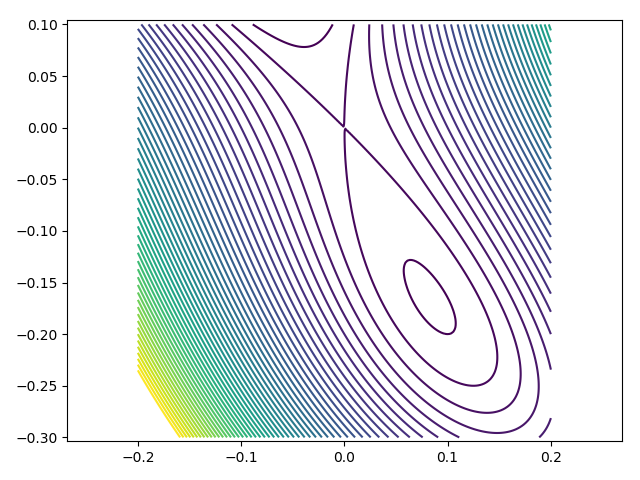
\includegraphics[scale=\myscale,scale=0.7]{figures/gradient-surface-6}
\end{center}

\end{exemple}
Sur l'exemple précédent, nous avons assez facilement calculé les points critiques à partir des deux équations à deux inconnues. Il faut prendre garde que ce n'est pas un système linéaire et que dans le cas d'une fonction plus compliquée il aurait été impossible de déterminer exactement les points critiques.

On note aussi dans l'exemple précédent que certains points critiques ne sont ni des maximums ni des minimums. L'exemple type, illustré ci-dessous, est celui d'un \defi{col} appelé aussi \defi{point-selle}\index{point-selle} en référence à sa forme de selle de cheval.

\begin{exemple}
Soit $f(x,y)=x^2-y^2$.
Voici son graphe vu sous trois angles différents et ses lignes de niveau.

\begin{center}
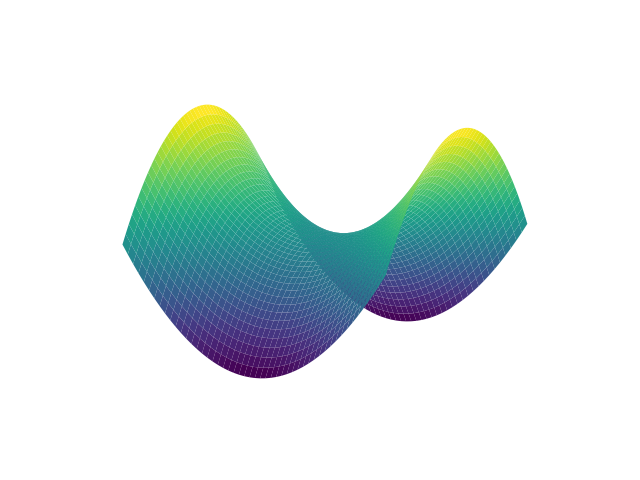
\includegraphics[scale=\myscale,scale=0.7]{figures/gradient-surface-3a}
\end{center}
\begin{center}
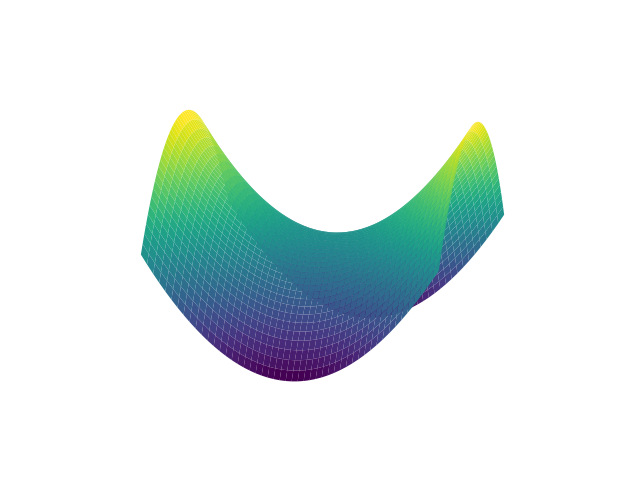
\includegraphics[scale=\myscale,scale=0.5]{figures/gradient-surface-3b}
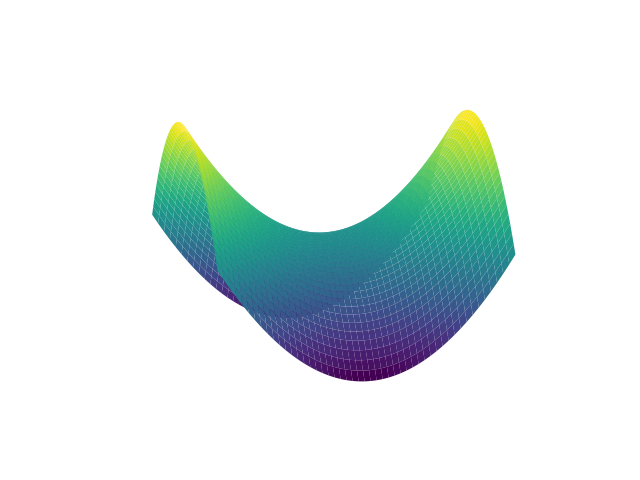
\includegraphics[scale=\myscale,scale=0.5]{figures/gradient-surface-3c}
\end{center}
\begin{center}
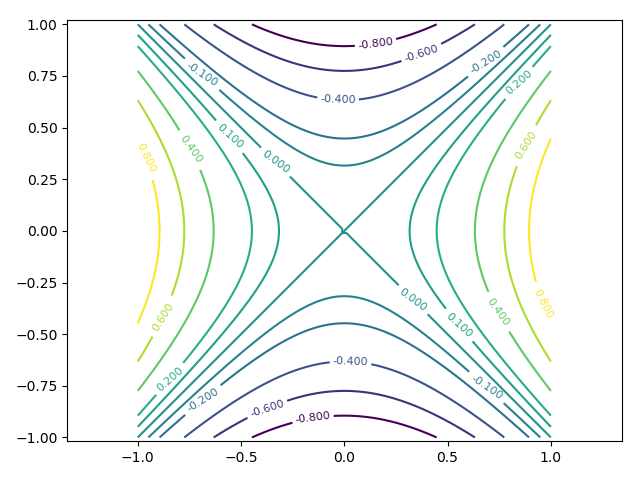
\includegraphics[scale=\myscale,scale=0.7]{figures/gradient-surface-4}
\end{center}


\end{exemple}


Comme il peut être difficile de calculer les points critiques de façon exacte, nous allons utiliser des méthodes numériques.
L'idée qui sera détaillée dans le prochain chapitre est la suivante : comme le gradient indique la direction dans laquelle la fonction $f$ croît le plus rapidement, nous allons suivre la direction opposée au gradient, pour laquelle $f$ décroît le plus rapidement. Ainsi, partant d'un point $(x_0,y_0)$ au hasard, on sait dans quelle direction se déplacer pour obtenir un nouveau point $(x_1,y_1)$ en lequel $f$ est plus petite. Et on recommence.

Sur les trois dessins ci-dessous, on a dessiné les lignes de niveau d'une fonction $f$ ainsi que les vecteurs $-\grad f(x,y)$. On voit que ces vecteurs pointent bien vers le minimum (figure de gauche), s'éloignent d'un maximum (figure centrale), le cas d'un point-selle est spécial (figure de droite). Dans tous les cas, la longueur des vecteurs gradients diminue à l'approche du point critique.


\begin{center}
\begin{minipage}{0.30\textwidth}
\center
\ \ 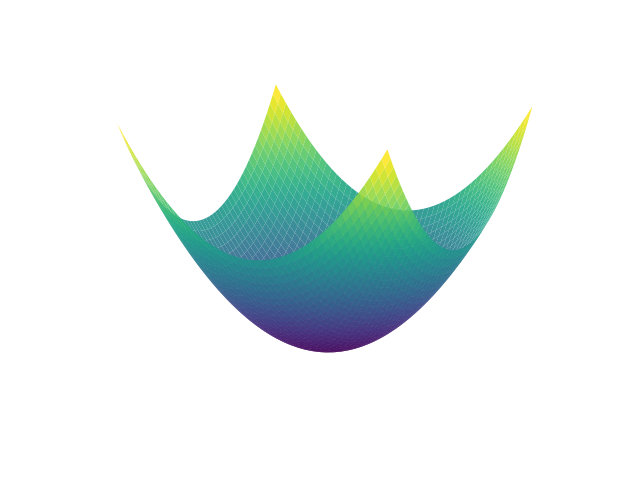
\includegraphics[scale=\myscale,scale=0.35]{figures/gradient-surface-1b}\\

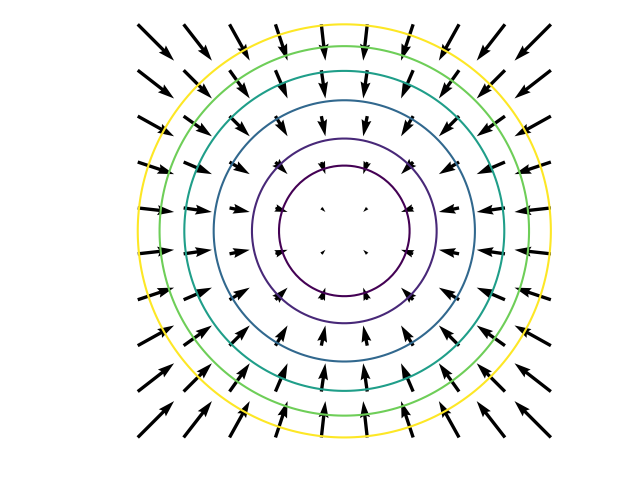
\includegraphics[scale=\myscale,scale=0.35]{figures/gradient-surface-5a}

\quad\textbf{Cas d'un minimum}
\end{minipage}
\begin{minipage}{0.30\textwidth}
  \center

  \ \ 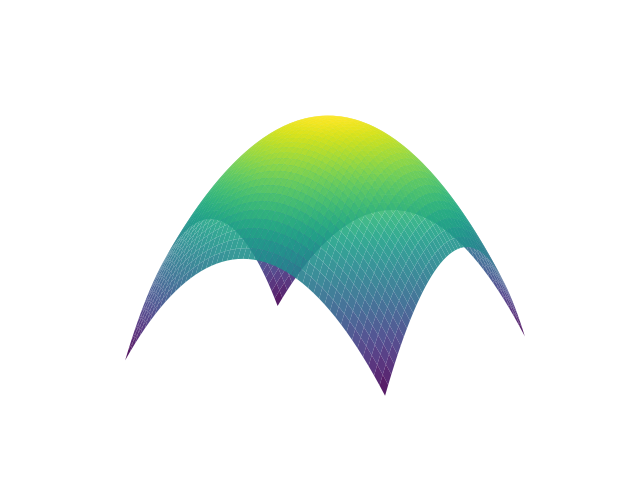
\includegraphics[scale=\myscale,scale=0.35]{figures/gradient-surface-2}\\

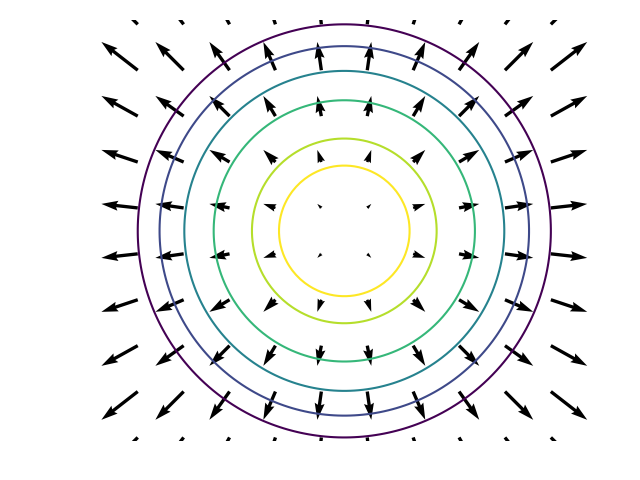
\includegraphics[scale=\myscale,scale=0.35]{figures/gradient-surface-5b}

\quad\textbf{Cas d'un maximum}
\end{minipage}
\begin{minipage}{0.30\textwidth}
\center
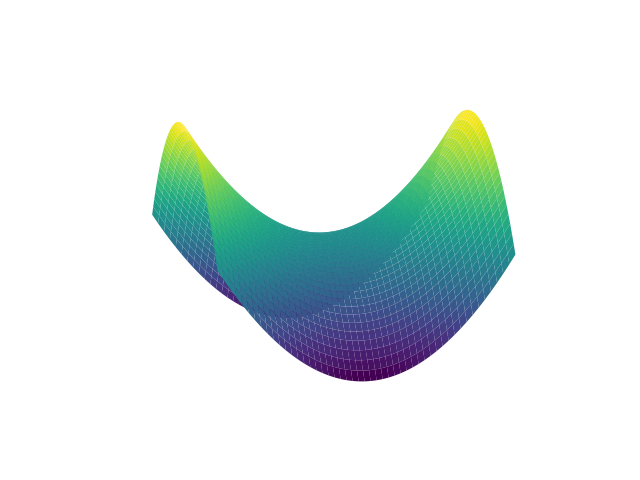
\includegraphics[scale=\myscale,scale=0.35]{figures/gradient-surface-3c}\\

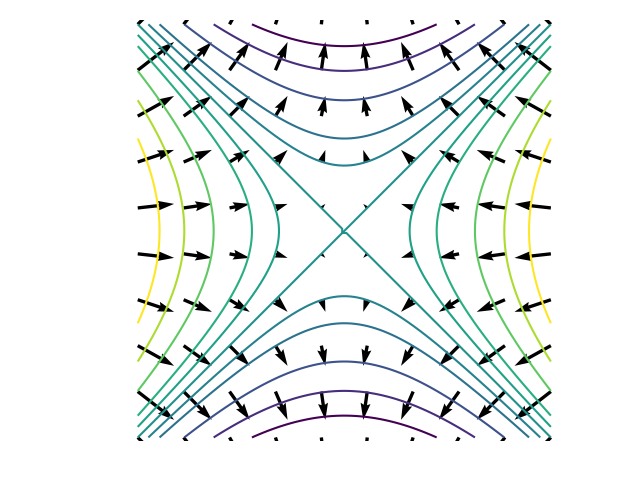
\includegraphics[scale=\myscale,scale=0.35]{figures/gradient-surface-5c}

\quad\textbf{Cas d'un point-selle}
\end{minipage}
\end{center}

%%%%%%%%%%%%%%%%%%%%%%%%%%%%%%%%%%%%%%%%%%%%%%%%%%%%%%%%%%%%%%%%%%%%%
\section{Différentiation automatique}

\index{différentiation automatique}

Dans le chapitre \og{}Dérivée\fg{}, nous avons vu comment calculer la dérivée d'une fonction composée à l'aide de son graphe de calcul. Nous allons faire de même pour les dérivées partielles des fonctions de plusieurs variables afin de calculer le gradient d'une fonction définie par un réseau de neurones.

%--------------------------------------------------------------------
\subsection{Différentiation automatique}

\textbf{Graphe de calcul.}\index{graphe de calcul}
Voici le graphe de calcul d'une fonction $f$ de deux variables (schéma de principe à gauche, évaluation en $(x_0,y_0)$ à droite).

\myfigure{0.6}{
\tikzinput{fig-diffauto-01}\qquad\qquad\qquad
\tikzinput{fig-diffauto-02}
}


\bigskip
\textbf{Dérivées locales.}
Voici la règle pour les dérivées locales à rajouter à chaque branche (entre crochets).
\myfigure{0.6}{
\tikzinput{fig-diffauto-03}
}
On note $\partial_x f$ comme raccourci de la fonction $\frac{\partial f}{\partial x}$.


\bigskip
\textbf{Dérivées partielles.}
On obtient chacune des dérivées partielles d'une composition $F$ comme le produit des dérivées locales le long des branches allant de la sortie $F(x,y)$ vers l'entrée $x$ (ou $y$).
\myfigure{0.8}{
\tikzinput{fig-diffauto-04}
}


\bigskip
\textbf{Formule mathématique.}
Soit $f : \Rr^2 \to \Rr$ et $g : \Rr \to \Rr$. 

\myfigure{0.6}{
\tikzinput{fig-diffauto-05}
}
La composition $F = g \circ f : \Rr^2 \to \Rr$ correspond au graphe de calcul dessiné ci-dessous :
\myfigure{0.6}{
\tikzinput{fig-diffauto-06}
}

On a donc :
$$F(x,y) = g \circ f (x,y) = g \big( f(x,y) \big).$$
Les dérivées partielles de $F$ sont données par les formules :
\mybox{$\displaystyle
\begin{array}{c}
\displaystyle \frac{\partial F}{\partial x}(x_0,y_0) = \frac{\partial f}{\partial x}(x_0,y_0) \cdot g'\big(f(x_0,y_0)\big)\\[4ex]
\displaystyle \frac{\partial F}{\partial y}(x_0,y_0) = \frac{\partial f}{\partial y}(x_0,y_0) \cdot g'\big(f(x_0,y_0)\big)
\end{array}
$}

La preuve de la formule pour $\frac{\partial F}{\partial x}(x_0,y_0)$ découle directement de la formule de la dérivée d'une composition pour la fonction d'une seule variable $x \mapsto F(x,y_0)$. Il en est de même pour l'autre dérivée partielle.
Ces formules justifient notre règle de calcul : la dérivée partielle est le produit des dérivées locales le long de chacune des branches.

\myfigure{0.8}{
\tikzinput{fig-diffauto-07}
}


\bigskip
\textbf{Addition et multiplication.}

Dans le cas $f(x,y) = x + y$ et $f(x,y)= x \times y$, on retrouve les dérivées locales déjà utilisées dans le cas d'une seule variable.

\myfigure{0.6}{
\tikzinput{fig-diffauto-08}\qquad\qquad\qquad
\tikzinput{fig-diffauto-09}
}



\bigskip
\textbf{Exemple.}
Soit $F(x,y) = \ln(x^2y+\sin y)$. On souhaite calculer $\grad F(3,2)$.
Nous allons montrer comment calculer $\grad F(x_0,y_0)$ pour $x_0$ et $y_0$ quelconques, puis nous reprendrons les calculs depuis le début dans le cas $(x_0,y_0)=(3,2)$.

\myfigure{0.8}{
\tikzinput{fig-diffauto-10}
}
\myfigure{0.8}{
\tikzinput{fig-diffauto-11}
}

On obtient les dérivées partielles comme produit des dérivées locales :
$$\frac{\partial F}{\partial x} (x_0,y_0) = \left[ \frac{1}{z_0} \right] \times [2x_0y_0] = \frac{2x_0y_0}{x_0^2y_0+\sin y_0},$$
$$\frac{\partial F}{\partial y} (x_0,y_0) = \left[ \frac{1}{z_0} \right] \times [x_0^2 + \cos y_0] = \frac{x_0^2 + \cos y_0}{x_0^2y_0+\sin y_0}.$$



Dans la pratique, pour les réseaux de neurones, on ne calcule jamais l'expression formelle de $\grad F(x_0,y_0)$ mais seulement des gradients en des valeurs $(x_0,y_0)$ données. On reprend donc à chaque fois les étapes ci-dessus mais uniquement pour des valeurs numériques.



La première étape est de calculer les valeurs des fonctions (de la gauche vers la droite).
\myfigure{0.8}{
\tikzinput{fig-diffauto-12}
}

La seconde étape est de calculer toutes les dérivées locales. On utilise les valeurs de l'étape précédente et la connaissance des formules de chacune des dérivées des fonctions élémentaires (ici $\frac{\partial f}{\partial x}$, $\frac{\partial f}{\partial y}$ et $\frac{\dd \ln}{\dd z}$).

\myfigure{0.8}{
\tikzinput{fig-diffauto-13}
}

On calcule le produit des dérivées locales le long des arêtes. 
\myfigure{0.8}{
\tikzinput{fig-diffauto-14}
}

On obtient les dérivées partielles :
{\small
$$\frac{\partial F}{\partial x} (3,2) = \left[ \frac{1}{18+\sin 2} \right] \times [12] = \frac{12}{18 + \sin 2}
\qquad \text{ et } \qquad 
\frac{\partial F}{\partial y} (3,2) = \left[ \frac{1}{18+\sin 2} \right] \times [9 + \cos 2] = \frac{9 + \cos 2}{18+\sin 2}.$$
}

\bigskip
\textbf{Règle générale.}
Dans le cas de $n$ entrées $(x_1,\ldots,x_n)$, la règle des dérivées locales se généralise naturellement : on associe à la branche numéro $i$ la dérivée locale $\frac{\partial f}{\partial x_i}$.

\myfigure{0.8}{
\tikzinput{fig-diffauto-15}
}


%--------------------------------------------------------------------
\subsection{Différentiation automatique (suite)}


\textbf{Graphe de calcul.}
Voici le graphe de calcul d'une situation que l'on a déjà rencontrée dans le cas d'une seule variable, mais dont la formule se justifie par les fonctions de deux variables.
Il s'agit du graphe de calcul de $F(t) = f\big( u(t), v(t) \big)$ où
$u : \Rr \to \Rr$, $v : \Rr \to \Rr$ et $f : \Rr^2 \to \Rr$. L'objectif est de calculer $F'(t)$.

\myfigure{0.55}{
\tikzinput{fig-diffauto-21}\qquad
\tikzinput{fig-diffauto-22}
}

\bigskip
\textbf{Dérivées locales.}
On calcule les dérivées locales comme d'habitude.
\myfigure{0.8}{
\tikzinput{fig-diffauto-23}
}

\bigskip
\textbf{Dérivée.}
La dérivée s'obtient en deux étapes :
\begin{itemize}
  \item on calcule le produit des dérivées locales le long des chemins partant de chaque arête sortante jusqu'à la sortie,
  \item puis on calcule la somme de ces produits.
\end{itemize}

\myfigure{0.9}{
\tikzinput{fig-diffauto-24}
}

\bigskip
\textbf{Formule mathématique.}
La situation est cette fois la suivante :
\myfigure{0.6}{
\tikzinput{fig-diffauto-25}
}
La formule de dérivation de la composition de
$$F(t) = f\big( u(t), v(t) \big)$$
est :
\mybox{$\displaystyle
F'(t_0) = u'(t_0) \frac{\partial f}{\partial x}(u(t_0),v(t_0)) \  + \  v'(t_0) \frac{\partial f}{\partial y}(u(t_0),v(t_0)) 
$}


\bigskip
\textbf{Exemple.}
Soit $F(t) = \sqrt{\exp(t)\sin(t)}$. On souhaite calculer $F'(1)$. On commence par calculer $F'(t_0)$ en général avant de tout reprendre dans la cas $t_0=1$.
Voici le graphe de calcul :
\myfigure{0.6}{
\tikzinput{fig-diffauto-26}
}
Une fois complété avec les dérivées locales cela donne :
\myfigure{0.8}{
\tikzinput{fig-diffauto-27}
}
On trouve ainsi :
$$F'(t_0) = \left[\frac{1}{2\sqrt{z_0}}\right]\cdot[y_0]\cdot[\exp t_0]
\  + \  \left[\frac{1}{2\sqrt{z_0}}\right]\cdot[x_0]\cdot[\cos t_0]
$$
et donc 
$$F'(t_0) = \frac{\exp t_0 \cdot (\sin t_0 + \cos t_0)}{2\sqrt{\exp t_0 \sin t_0}}.$$

Reprenons tout depuis le début pour calculer $F'(1)$ en oubliant que l'on a déjà trouvé la formule générale :
\myfigure{0.8}{
\tikzinput{fig-diffauto-28}
}
On trouve ainsi :
$$F'(1) = \left[\frac{1}{2\sqrt{e\sin(1)}}\right]\cdot[\sin(1)]\cdot[e]
\  + \  \left[\frac{1}{2\sqrt{e\sin(1)}}\right]\cdot[e]\cdot[\cos(1)]
$$
et donc 
$$F'(1) = \frac{e (\sin(1)+\cos(1))}{2\sqrt{e\sin(1)}}.$$


\bigskip
\textbf{Règle générale.}
Dans le cas de $n$ sorties, on somme sur toutes les arêtes sortantes comme dans la situation ci-dessous.
\myfigure{0.8}{
\tikzinput{fig-diffauto-29}
}
La fonction est $F(t) = t + (\ln t)^2 + \frac{1}{\sin t}$ et en sommant on trouve bien $F'(t) = 1 + \frac{2\ln t}{t} - \frac{\cos t}{\sin^2 t}$.


\bigskip
\textbf{Un autre exemple.}
On termine par un exemple plus compliqué : on souhaite calculer la dérivée de 
$$F(t) = t^2 \cdot \ln t \cdot \ln(\ln t).$$
Voici le graphe de calcul que l'on utilise (noter qu'avec ce graphe, on ne calcule qu'une seule fois $\ln t$ dont le résultat est réutilisé pour calculer $\ln(\ln t)$).

\myfigure{0.8}{
\tikzinput{fig-diffauto-30}
}

La dérivée s'obtient comme somme sur tous les chemins de la sortie à l'entrée.
C'est donc un peu plus compliqué que ce l'on pense au premier abord : il faut ici faire la somme selon trois chemins différents, car l'arête sortant de la variable $t$ vers la variable $y$ se sépare ensuite en deux. Nous allons voir comment gérer cette difficulté dans la section suivante.


%%%%%%%%%%%%%%%%%%%%%%%%%%%%%%%%%%%%%%%%%%%%%%%%%%%%%%%%%%%%%%%%%%%%%
\section{Gradient pour un réseau de neurones}

%--------------------------------------------------------------------
\subsection{Fonction associée à un réseau}
\label{ssec:foncres}

Pour un réseau de neurones $\mathcal{R}$ ayant $n$ entrées $(x_1,\ldots,x_n)$ et une seule sortie, nous associons une fonction : $F : \Rr^n \to \Rr$,  $(x_1,\ldots,x_n) \mapsto F(x_1,\ldots,x_n)$. La situation est en fait plus compliquée. Jusqu'ici les paramètres du réseau étaient donnés. \`A partir de maintenant les variables du problème ne seront plus les entrées mais les poids du réseau. 
Notons $a_1,\ldots,a_m$ ces poids (l'ensemble des coefficients et des biais). Si l'entrée est fixée et que les poids sont les variables du réseau alors on pourrait considérer que ce même réseau $\mathcal{R}$ définit la fonction 
$\widetilde F : \Rr^m \to \Rr$, $(a_1,\ldots,a_m) \mapsto \widetilde F(a_1,\ldots,a_m)$. 

\myfigure{0.6}{
\tikzinput{fig-gradres-01}
}


Ce dont nous aurons besoin pour la suite et que nous allons calculer dans ce chapitre c'est le gradient de $\widetilde F$ par rapport aux poids $(a_1,\ldots,a_m)$, autrement dit, il s'agit de calculer :
$$\frac{\partial \widetilde F}{\partial a_j}.$$

Pour concilier les deux points de vue (entrées et poids), on dira qu'un réseau de neurones ayant des entrées $(x_1,\ldots,x_n)$ et des poids 
$(a_1,\ldots,a_m)$ définit la fonction :
$$\begin{array}{lccc}
\widehat F : & \Rr^n             \times  \Rr^m & \longrightarrow & \Rr \\
    & (x_1,\ldots,x_n)  ,  (a_1,\ldots,a_m) & \longmapsto & \widehat F(x_1,\ldots,x_n,a_1,\ldots,a_m) \\
\end{array}$$

\begin{remarque*}
Ce n'est pas tout à fait la fonction $\widetilde F$ dont on voudra calculer le gradient mais notre attention se portera sur une fonction d'erreur $E$ de la forme
$E = (\widetilde F-y_0)^2$, où $\widetilde F$ est la fonction définie ci-dessus correspondant à une certaine entrée et à la sortie $y_0$.
On calcule facilement les dérivées partielles de $E$ à partir de celles de $\widetilde F$ par la formule :
$$\frac{\partial E}{\partial a_j} = 2\frac{\partial \widetilde F}{\partial a_j}(\widetilde F-y_0).$$
Voir le chapitre \og{}Rétropropagation\fg{} pour plus de détails.
\end{remarque*}


%--------------------------------------------------------------------
\subsection{Formule du gradient}

On considère la portion suivante d'un réseau de neurones :
\myfigure{1}{
\tikzinput{fig-gradres-02}
}
On s'intéresse à une seule arête entrante du neurone central\couleurnb{ rouge}{}, celle qui porte le poids $a$.
\begin{itemize}
  \item $a$ et $b$ sont des poids,
  \item $f, g, h$ sont des fonctions d'activation,
  \item $f', g', h'$ sont leur dérivées,
  \item $F$ est la fonction associée au réseau complet.
\end{itemize}

Pour distinguer la fonction de sa valeur en un point, on notera $f$ la fonction et $f_\mystar$ la valeur de la fonction à la sortie du neurone correspondant.

Voici la formule pour calculer la dérivée partielle de $F$ par rapport au coefficient $a$, connaissant la dérivée partielle par rapport au coefficient $b$.
\mybox{$\displaystyle
\frac{\partial F}{\partial a} = f_\mystar \cdot \frac{g'_\mystar}{g_\mystar} \cdot b \cdot \frac{\partial F}{\partial b}
$} 
Voici un schéma pour retenir cette \og{}\defi{formule du sourire}\fg{}\index{formule du sourire}:
on multiplie les coefficients $f_\mystar$, $g'_\mystar$, $b$ et la dérivée partielle par rapport à $b$ le long de l'arc et on divise par le coefficient $g_\mystar$ au bout du segment.
\myfigure{1.4}{
\tikzinput{fig-gradres-03}
}
Il est à noter que dans la formule, seule l'arête portant le coefficient $a$ intervient, les autres arêtes entrantes n'interviennent pas (et ne sont pas représentées). 
Par contre, dans le cas de plusieurs arêtes sortantes il faut calculer la somme 
des formules précédentes sur chaque arête :
\mybox{$\displaystyle
\frac{\partial F}{\partial a} = \sum_{i=1}^{\ell} f_\mystar \cdot \frac{g'_\mystar}{g_\mystar} \cdot b_{i} \cdot \frac{\partial F}{\partial b_i}
$} 
Cette somme comporte autant de termes que d'arêtes sortantes (il n'y a pas à énumérer tous les chemins entre le sommet et la sortie comme auparavant dans la différentiation automatique).
\myfigure{1}{
\tikzinput{fig-gradres-04}
}

\bigskip

Pour pouvoir calculer toutes les dérivées partielles, on procède par récurrence, en partant de la fin puis en revenant en arrière de proche en proche. 

\myfigure{1}{
\tikzinput{fig-gradres-05}
}

Voici la formule d'initialisation associée aux coefficients en sortie de réseau, dite \og{}formule du demi-sourire\fg{} :
\mybox{$\displaystyle
\frac{\partial F}{\partial a} = f_\mystar \cdot g'_\mystar
$} 


\bigskip

Voici quelques situations particulières, mais qui sont simplement des applications de la formule du sourire.

\textbf{Formule à l'entrée.} On applique la formule du sourire avec $x$ à la place de $f$.
$$\frac{\partial F}{\partial a} = x \cdot \frac{g'_\mystar}{g_\mystar} \cdot b \cdot \frac{\partial F}{\partial b}$$ 
\myfigure{1}{
\tikzinput{fig-gradres-06}
}

\textbf{Dérivée partielle par rapport aux variables d'entrées.}
On applique la formule du sourire en ajoutant des coefficients virtuels égaux à $1$ (la dérivée de $x$ par rapport à $x$ est $1$) :
$$\frac{\partial F}{\partial x} = \frac{b}{x} \cdot \frac{\partial F}{\partial b}$$
\myfigure{1}{
\tikzinput{fig-gradres-07}
}


\textbf{Cas d'un biais.} On applique la formule du sourire en ajoutant un coefficient virtuel égal à $1$ :
$$\frac{\partial F}{\partial a} = \frac{g'_\mystar}{g_\mystar} \cdot b \cdot \frac{\partial F}{\partial b}$$ 
\myfigure{1}{
\tikzinput{fig-gradres-08}
}


\begin{remarque*}
\sauteligne
\begin{itemize}
  \item Ces formules ne sont pas valables lorsque $g_\star=0$. Nous verrons lors de la preuve de ces formules comment régler ce problème.
  
  \item Il faut s'habituer au jeu d'écriture un peu ambigu, comme on le fait pour une expression $y$ qui dépend de $x$. On peut noter cette expression $y(x)$ ou bien simplement $y$, cette dernière écriture peut désigner une fonction de $x$ ou bien la valeur prise en $x$. Par exemple dans la formule du sourire  $\frac{\partial F}{\partial a}$ et $ \frac{\partial F}{\partial b}$ sont en fait les valeurs des dérivées partielles et ne sont pas vraiment considérées comme des fonctions. Dans la pratique cela ne posera pas de problème car le but est de calculer les valeurs des dérivées partielles (et pas l'expression des fonctions dérivées partielles).
  
  \item De plus, les expressions sont dérivées par rapport à différentes variables. Par exemple, si une expression $F$ dépend de $y$, et l'expression $y$ dépend de $x$, alors on peut calculer  $\frac{\partial F}{\partial y}$, mais aussi $\frac{\partial F}{\partial x}$. 
  
  \item Enfin la fonction $F$ considérée ici dépend des variables d'entrée $x_i$ mais aussi des poids $a_j$, si on suivait le formalisme introduit en section \ref{ssec:foncres}, on devrait plutôt la noter  $\widehat F$.
\end{itemize}
\end{remarque*}


%--------------------------------------------------------------------
\subsection{Premier exemple}

Voici un réseau très simple.
\myfigure{1}{
\tikzinput{fig-gradres-09}
}
Avec :
\begin{itemize}
  \item une entrée $x$, une sortie $F(x)$,
  \item trois poids $a,b,c$,
  \item des fonctions d'activation (plutôt fantaisistes) $u \mapsto u^2$ et $v \mapsto \ln v$.
\end{itemize}
Nous avions l'habitude de considérer la fonction $x \mapsto F(x)$ mais dorénavant les poids sont de nouvelles variables, nous devons donc étudier la fonction 
$\widehat F$ introduite ci-dessus que nous noterons encore $F$ dans la suite :
$$F(x,a,b,c) = \ln\big( c (ax+b)^2 \big).$$
Nous souhaitons calculer les dérivées partielles de $F$ par rapport aux poids $a,b,c$. Nous ne souhaitons pas obtenir une formule générale mais juste la valeur exacte de ces dérivées partielles en un point précis. Nous choisissons l'exemple de 
$(x,a,b,c) = (2,3,4,5)$.
On récrit le réseau avec les valeurs des poids, les valeurs des fonctions et les valeurs des dérivées locales.
\myfigure{1}{
\tikzinput{fig-gradres-10}
}


\textbf{Calcul de la dérivée partielle par rapport à $c$.}
On part de la sortie pour l'initialisation. On applique la formule du demi-sourire.
\myfigure{1}{
\tikzinput{fig-gradres-11}
}
$$\frac{\partial F}{\partial c} = 100 \times \frac{1}{500} = \frac15.$$

\textbf{Calcul de la dérivée partielle par rapport à $a$.}
On applique la formule du sourire :
$$\frac{\partial F}{\partial a} = 2 \times \frac{20}{100} \times 5 \times \frac{\partial F}{\partial c}.$$
\myfigure{1}{
\tikzinput{fig-gradres-12}
}
Mais on a déjà calculé $\frac{\partial F}{\partial c}=\frac15$ (entre accolades doubles), donc :
$$\frac{\partial F}{\partial a} = \frac25.$$

\textbf{Calcul de la dérivée partielle par rapport à $b$.}
On applique la formule du sourire (en posant $1$ pour le coefficient manquant):
$$\frac{\partial F}{\partial b} = 1 \times \frac{20}{100} \times 5 \times \frac{\partial F}{\partial c}.$$
\myfigure{1}{
\tikzinput{fig-gradres-13}
}
Donc 
$$\frac{\partial F}{\partial b} = \frac15.$$

\textbf{Calcul de la dérivée partielle par rapport à $x$.}
On peut aussi calculer cette dérivée partielle, même si nous n'en aurons pas besoin dans les autres chapitres. 
$$\frac{\partial F}{\partial x} = 1 \times \frac{1}{2} \times 3 \times \frac{\partial F}{\partial a}.$$
\myfigure{1}{
\tikzinput{fig-gradres-14}
}
donc 
$$\frac{\partial F}{\partial x} = \frac{3}{5}.$$

\textbf{Bilan.}
Ainsi $F(2,3,4,5)=\ln 500$ et on a calculé les dérivées partielles (entre doubles accolades) pour chacune des variables $x,a,b,c$.
\myfigure{1}{
\tikzinput{fig-gradres-15}
}

\textbf{Vérification.}
On peut vérifier nos formules en calculant directement les dérivées partielles à partir de l'expression :
$$F(x,a,b,c) = \ln\big( c (ax+b)^2 \big).$$
Par exemple :
$$\frac{\partial F}{\partial a}(x,a,b,c) = \frac{2cx(ax+b)}{c(ax+b)^2} = \frac{2x}{ax+b}$$
et on a bien 
$$\frac{\partial F}{\partial a}(2,3,4,5) = \frac{4}{10} = \frac25.$$

%--------------------------------------------------------------------
\subsection{Second exemple}

Pour le réseau suivant, on associe comme précédemment une fonction $F$. 
\myfigure{1}{
\tikzinput{fig-gradres-16}
}
On considère les poids $a,b,c,d$ comme des variables, la fonction $F : \Rr^5 \to \Rr$ s'écrit donc :
$$F(x,a,b,c,d) = \exp\big(c \cos(ax) + d\sin(bx)\big).$$

On va noter $u=ax$ et $v=bx$, ainsi $\cos u$ et $\sin v$ sont les sorties des deux premiers neurones. On note $w =c\cos u + d\sin v$. La sortie du troisième neurone (qui est aussi la valeur de $F$) est alors $\exp w$.

On part de la sortie pour l'initialisation. Il y a deux dérivées partielles à calculer.

\textbf{Calcul de la dérivée partielle par rapport à $c$.}
On applique la formule du demi-sourire :
$$\frac{\partial F}{\partial c} = \cos u \cdot \exp w.$$

\textbf{Calcul de la dérivée partielle par rapport à $d$.}
On applique de nouveau la formule du demi-sourire :
$$\frac{\partial F}{\partial d} = \sin v \cdot \exp w.$$

\textbf{Calcul de la dérivée partielle par rapport à $a$.}
On applique la formule du sourire :
$$\frac{\partial F}{\partial a} = x \cdot \frac{-\sin u}{\cos u} \cdot c \cdot  \frac{\partial F}{\partial c}$$
donc 
$$\frac{\partial F}{\partial a} = -x c \sin u \exp w.$$

\textbf{Calcul de la dérivée partielle par rapport à $b$.}
On applique la formule du sourire :
$$\frac{\partial F}{\partial b} = x \cdot \frac{\cos v}{\sin v} \cdot d \cdot  \frac{\partial F}{\partial d}$$
donc 
$$\frac{\partial F}{\partial b} = x d \cos v \exp w.$$

\textbf{Calcul de la dérivée partielle par rapport à $x$.}
Cette dérivée partielle s'obtient comme la somme de deux termes correspondant aux deux arêtes sortantes :
$$\frac{\partial F}{\partial x} = a \cdot \frac{1}{x} \cdot \frac{\partial F}{\partial a} \ + \  b \cdot \frac{1}{x} \cdot \frac{\partial F}{\partial b}$$
donc 
$$\frac{\partial F}{\partial x} = (-ac\sin u + bd\cos v) \exp w.$$

\textbf{Vérification.}
En effectuant les substitutions $u=ax$, $v=bx$ et $w =c\cos (ax) + d\sin (bx)$,
on retrouve les dérivées partielles attendues, par exemple
$$\frac{\partial F}{\partial x} = \big(-ac\sin (ax) + bd\cos (bx) \big) \exp \big(c\cos (ax) + d\sin (bx) \big).$$

%--------------------------------------------------------------------
\subsection{Preuve et formule générale}

\myfigure{1}{
\tikzinput{fig-gradres-17}
}

\textbf{Préliminaires.}

\mybox{
  \begin{equation}
    \frac{\partial h}{\partial g} = b \cdot h'_\mystar
    \label{eq:grad:eq1}
  \end{equation}
}
Preuve : on a $h_\mystar = h(b g_\mystar)$, la formule s'obtient en dérivant $g \mapsto h(bg)$ par rapport à la variable $g$, avec 
$h'_\mystar = h'(b g_\mystar)$.

\mybox{
  \begin{equation}
    \frac{\partial g}{\partial a} = f_\mystar \cdot g'_\mystar
    \label{eq:grad:eq2}
  \end{equation}
}
Preuve : on a $g_\mystar = g(\cdots + a f_\mystar+\cdots)$, la formule s'obtient en dérivant $a \mapsto g(\cdots + a f +\cdots)$ par rapport à la variable $a$. On note $g'_\mystar = g'(\cdots + a f_\mystar+\cdots)$.

\mybox{
  \begin{equation}
    \frac{\partial h}{\partial b} = g_\mystar \cdot h'_\mystar
    \label{eq:grad:eq3}
  \end{equation}
  }
Preuve : c'est la même formule que l'équation (\ref{eq:grad:eq2}) mais cette fois pour $b \mapsto h(b g)$ et $h'_\mystar = h'(b g_\mystar)$.

\bigskip
\textbf{Formule générale.}

\mybox{
    \begin{equation}
      \frac{\partial F}{\partial a} = \frac{\partial F}{\partial g} \cdot f_\mystar \cdot  g'_\mystar
      \label{eq:grad:eq4}
    \end{equation}
}

Preuve :
c'est la formule
$$\frac{\partial F}{\partial a} =  \frac{\partial F}{\partial g} \cdot \frac{\partial g}{\partial a}$$
(valable car $g$ est une fonction d'une seule variable) suivie de l'application de l'équation (\ref{eq:grad:eq2}).

\mybox{
\begin{equation}
\frac{\partial F}{\partial g} = \frac{\partial F}{\partial h} \cdot b \cdot  h'_\mystar
\label{eq:grad:eq5}
\end{equation}
}

Preuve :
c'est la formule
$$\frac{\partial F}{\partial g} =  \frac{\partial F}{\partial h} \cdot \frac{\partial h}{\partial g}$$
suivie de l'application de l'équation (\ref{eq:grad:eq1}).

Dans le cas d'un neurone de sortie on a :
\mybox{
\begin{equation}
\frac{\partial F}{\partial g} = 1
\label{eq:grad:eq6}
\end{equation}
}
car comme $g$ est la dernière fonction, on a $F_\mystar = g_\mystar$.

\bigskip
\textbf{Algorithme.}


\myfigure{1}{
\tikzinput{fig-gradres-18}
}
Voici comment calculer toutes les dérivées partielles voulues (y compris dans le cas $g_\mystar=0$ qui avait été exclu dans la formule du sourire).
\begin{itemize}
  \item On part du neurone de sortie pour lequel on initialise le processus par la formule
  (\ref{eq:grad:eq6}) ce qui donne 
  $\frac{\partial F}{\partial g_n} = 1$.
  \item On procède par récurrence à rebours. On suppose que l'on a déjà calculé
  $\frac{\partial F}{\partial g_{i+1}}$
  On en déduit :
  $$\frac{\partial F}{\partial g_{i}} =  \frac{\partial F}{\partial g_{i+1}} \cdot a_{i+1} \cdot  g'_{i+1,\mystar}$$
  par la formule (\ref{eq:grad:eq5}).
  \item Cela permet de calculer les dérivées partielles par rapport aux poids à l'aide de la formule (\ref{eq:grad:eq4}) :
  $$\frac{\partial F}{\partial a_i} = \frac{\partial F}{\partial g_i} \cdot g_{i-1,\mystar} \cdot  g'_{i,\mystar}.$$
\end{itemize}



\bigskip
\textbf{Preuve de la formule du sourire.}

On va exprimer $\frac{\partial F}{\partial a}$ directement en fonction de $\frac{\partial F}{\partial b}$.

Par les équations (\ref{eq:grad:eq4}) et (\ref{eq:grad:eq5}), on a d'une part :
\begin{equation}
\frac{\partial F}{\partial a} =   \frac{\partial F}{\partial h} \cdot b \cdot  h'_\mystar \cdot f_\mystar \cdot g'_\mystar
\label{eq:grad:eq7}
\end{equation}
et d'autre part :
$$\frac{\partial F}{\partial b} =  \frac{\partial F}{\partial h} \cdot \frac{\partial h}{\partial b}.$$
Donc, en utilisant l'équation (\ref{eq:grad:eq3}), on obtient :
\begin{equation}
\frac{\partial F}{\partial b} =   \frac{\partial F}{\partial h} \cdot g_\mystar \cdot  h'_\mystar.
\label{eq:grad:eq8}
\end{equation}
Cette dernière équation permet de calculer $\frac{\partial F}{\partial h}$ en fonction $\frac{\partial F}{\partial b}$. Ainsi des équations (\ref{eq:grad:eq7}) et (\ref{eq:grad:eq8}), on obtient la formule du sourire :
$$\frac{\partial F}{\partial a} = f_\mystar \cdot \frac{g'_\mystar}{g_\mystar} \cdot b \cdot \frac{\partial F}{\partial b}.$$

Dans le cas de plusieurs arêtes sortantes, il s'agit de faire une somme comme on l'a déjà vu lors de la différentiation automatique.


\end{document}
